\documentclass[ex,minted]{exercise}

\deadline{17.10.2023}

\begin{document}

\section{Tripelspiegel}
Da die Physik invariant unter Drehung und Translation des Raumes ist,
kann ohne Einschränkung der Allgemeinheit angenommen werden, dass 
die drei Flächennormalen die drei Einheitsvektoren sind.
\begin{align*}
    \vec b &= \vec a - 2 \vec n (\vec n \cdot \vec a)\\
    \\
    \vec b_1 &= \vec a - 2 \e_1 (\e_1 \cdot \vec a)\\
    &= \vec a - 2 \e_1 a_1\\
    &= \colvec{-a_1}{a_2}{a_3}\\
    \\
    \vec b_2 &= \vec b_1 - 2 \e_2 (\e_2 \cdot \vec b_1)\\
    &= \vec b_1 - 2 \e_2 a_2\\
    &= \colvec{-a_1}{-a_2}{a_3}\\
    \\
    \vec b_3 &= \vec b_2 - 2 \e_3 (\e_3 \cdot \vec b_2)\\
    &= \vec b_2 - 2 \e_3 a_3\\
    &= \colvec{-a_1}{-a_2}{-a_3}\\
    &= - \vec a
\end{align*}

\newpage
\section{Lichtkreis beim Tauchen}

\begin{figure}[h]
    \centering
    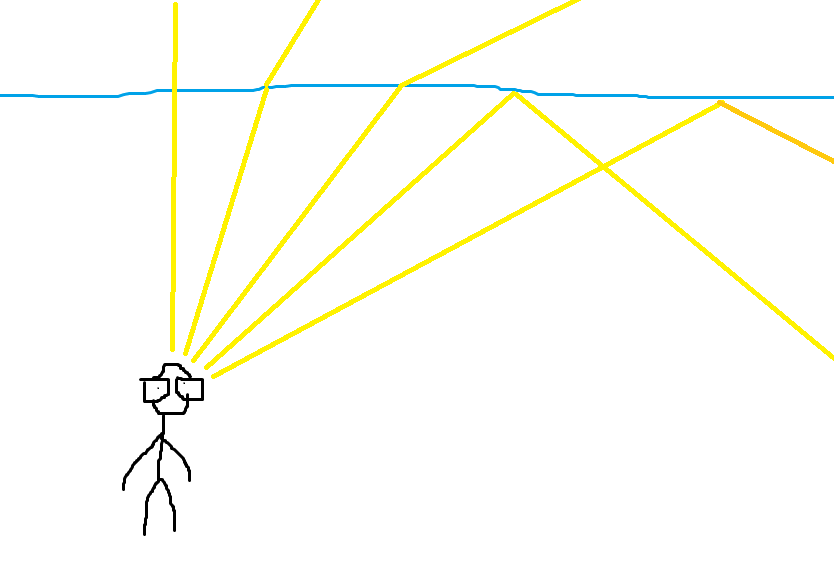
\includegraphics[width=0.4\textwidth]{1.png}
    \caption{Skizze eines Tauchers unter Wasser}
\end{figure}
\begin{align*}
    \frac{n_A}{n_B} &= \frac{\sin \beta}{\sin \alpha}\\
    \beta  &= \arcsin\hug{\frac{n_A}{n_B} \sin\alpha}\\
    &\approx \arcsin\hug{\frac1{1.\bar 3} \sin\frac \pi 2}\\
    &\approx 48.6^\circ\\
    \\
    \tan\hug{\frac\pi2 - \alpha} &= \frac{r}{h}\\
    r &= h \tan\hug{\frac\pi2 - \alpha}\\
    &\approx 10\u m \cdot \tan \hug{90^\circ - 48.6^\circ}\\
    &\approx 24.56 \u m
\end{align*}

\section{Lüneburg-Linse}
\begin{figure}[h]
    \centering
    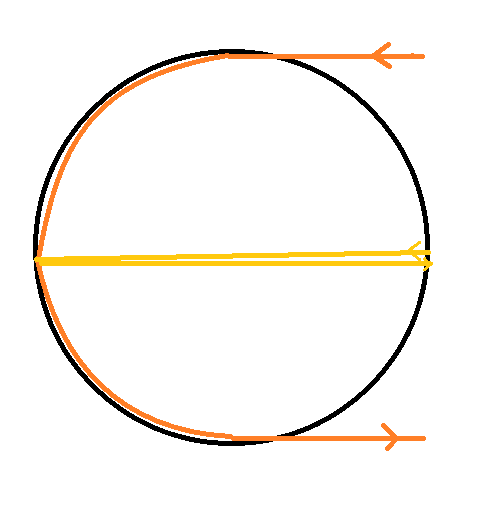
\includegraphics[width=0.35\textwidth]{4.png}
    \caption{Mittlerer und äußerer Lichtweg in der Lüneburg-Linse}
\end{figure}

\begin{align*}
    l_m &= \int n(\vec s(t)) \abs{\deriv{\vec s(t)}{t}} \dt\note 
    \vec s(t) = t\\
    &= 2\cdot \int_{-R}^{R} \sqrt{2-\hug{\frac tR}^2}\dt\\
    \subst[\dt = \sqrt2 R\du]{\sqrt2 u = \frac t{ R}}{t= \sqrt2 R u}\\
    &= 2\cdot \sqrt2 R \int_{-1}^{1} \sqrt{2-2u^2}\du\\
    &= 4 R \int_{-\frac1{\sqrt{2}}}^{\frac1{\sqrt{2}}} \sqrt{1-u^2}\du\\
    \subst[\du = \dv \cos v]{u = \sin v}{ v = \arcsin u}\\
    &= 4 R \int_{\arcsin-\frac1{\sqrt{2}}}^{\arcsin\frac1{\sqrt{2}}} \cos v \sqrt{1-\sin^2v}\dv\\
    &= 4 R \int_{\arcsin-\frac1{\sqrt{2}}}^{\arcsin\frac1{\sqrt{2}}} \cos^2 v\dv\\
    &= 4 R \int_{\arcsin-\frac1{\sqrt{2}}}^{\arcsin\frac1{\sqrt{2}}} \frac{\cos(2v)+1}{2}\dv\\
    &= 2R \hug{\half\sin(2v)+v}\eval_{\arcsin-\frac1{\sqrt{2}}}^{\arcsin\frac1{\sqrt{2}}}\\
    &\approx 5.14 R
\end{align*}

Außerster Lichtstrahl:
\begin{align*}
    l_a &= 2 R + \frac U2\\
    &= 2 R + \frac {2\pi R}2\\
    &= \hug{\pi + 2} R\\
    &\approx 5.14 R
\end{align*}
Insgesamt sind somit die beiden Lichtwege gleichlang.

\section{Regenbogen}
\begin{align*}
    \frac{n_A}{n_B} &= \frac{\sin \beta}{\sin \alpha}\\
    \beta  &= \arcsin\hug{\frac{n_A}{n_B} \sin\alpha}
\end{align*}
\begin{figure}[h]
    \centering
    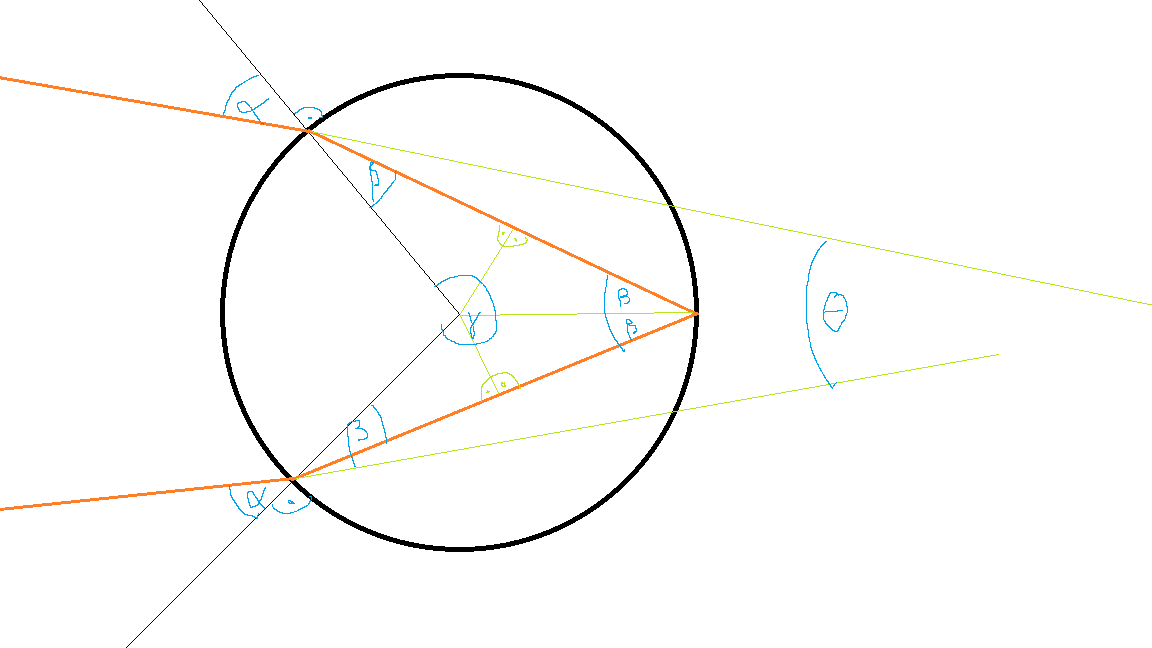
\includegraphics[width=0.7\textwidth]{3.png}
    \caption{Skizze der Geometrie im Regentropfen}
\end{figure}
\begin{align*}
    \begin{cases}
        \te I.\ \ 2\pi = 4\beta + \gamma\\
        \te{II}. \ 2\pi = 2\alpha + \gamma + \theta
    \end{cases}&\implies \theta =4\beta - 2 \alpha\\
    \theta &= 4 \arcsin\hug{\frac{n_A}{n_B} \sin\alpha} - 2 \alpha\\
    0 &= \deriv{\theta}{\alpha} \for \alpha_0\\
    &= \frac{4}{\sqrt{1 - \hug{\frac{n_A}{n_B} \sin\alpha_0}^2}}\frac{n_A}{n_B} \cos\alpha_0 -2\\
    1 -  \underbrace{\frac{n_A^2}{n_B^2}}_{=:c} \sin^2\alpha_0 &= \frac{4n_A^2}{n_B^2} \cos^2\alpha_0 \\
    1 &= c \sin^2\alpha_0 + 4 c \cos^2\alpha_0 \\
    1 &= \frac c2 \hug{1-\cos{2\alpha_0}} + 2 c \hug{1+\cos{2\alpha_0}} \\
    \frac1c - \frac 52 &= \frac 32 \cos{2\alpha_0} \\
    \alpha_0 &= \half\arccos\hug{\frac2{3c} - \frac{5}{3}}
    \note c=\frac{n_A^2}{n_B^2} \approx\frac{1^2}{\hug{\frac{4}{3}}^2}=\frac{9}{16}\\
    &\approx \half\arccos\hug{\frac{32}{27} - \frac{5}{3}}\\
    &= \half\arccos\hug{-\frac{13}{27}}\\
    &\approx 1.04 = 59.4 ^\circ\\
    \\
    \theta_0 &= 4\beta(\alpha_0) - 2\alpha_0\\
    &\approx 0.734 = 42.0^\circ
\end{align*}

\section{Lichtstrahl durch Atmosphäre}
\inputpy{Python code}{1.py}

\end{document}